%% LyX 2.2.3 created this file.  For more info, see http://www.lyx.org/.
%% Do not edit unless you really know what you are doing.
\documentclass[english]{article}
\usepackage[T1]{fontenc}
\usepackage[latin9]{inputenc}
\usepackage{geometry}
\geometry{verbose,tmargin=3cm,bmargin=3cm,lmargin=3cm,rmargin=3cm,headheight=3cm,headsep=3cm}
\usepackage{float}
\usepackage{graphicx}

\makeatletter

%%%%%%%%%%%%%%%%%%%%%%%%%%%%%% LyX specific LaTeX commands.
%% Because html converters don't know tabularnewline
\providecommand{\tabularnewline}{\\}

%%%%%%%%%%%%%%%%%%%%%%%%%%%%%% User specified LaTeX commands.
\usepackage{babel}

\makeatother

\usepackage{babel}
\begin{document}

\section{Ejercicio 4}

\begin{figure}[H]
\begin{centering}
\begin{tabular}{|c|c|c|c|c|c|c|c|}
\hline 
$x_{1}$  & $x_{2}$  & $x_{3}$  & $x_{4}$  & $f_{1}$  & $f_{2}$  & $f_{3}$  & $f_{4}$\tabularnewline
\hline 
\hline 
0  & 0  & 0  & 0  & 0  & 0  & 0  & 0\tabularnewline
\hline 
0  & 0  & 0  & 1  & 1  & 1  & 1  & 1\tabularnewline
\hline 
0  & 0  & 1  & 0  & 1  & 1  & 1  & 0\tabularnewline
\hline 
0  & 0  & 1  & 1  & 1  & 1  & 0  & 1\tabularnewline
\hline 
0  & 1  & 0  & 0  & 1  & 1  & 0  & 0\tabularnewline
\hline 
0  & 1  & 0  & 1  & 1  & 0  & 1  & 1\tabularnewline
\hline 
0  & 1  & 1  & 0  & 1  & 0  & 1  & 0\tabularnewline
\hline 
0  & 1  & 1  & 1  & 1  & 0  & 0  & 1\tabularnewline
\hline 
1  & 0  & 0  & 0  & 1  & 0  & 0  & 0\tabularnewline
\hline 
1  & 0  & 0  & 1  & 0  & 1  & 1  & 1\tabularnewline
\hline 
1  & 0  & 1  & 0  & 0  & 1  & 1  & 0\tabularnewline
\hline 
1  & 0  & 1  & 1  & 0  & 1  & 0  & 1\tabularnewline
\hline 
1  & 1  & 0  & 0  & 0  & 1  & 0  & 0\tabularnewline
\hline 
1  & 1  & 0  & 1  & 0  & 0  & 1  & 1\tabularnewline
\hline 
1  & 1  & 1  & 0  & 0  & 0  & 1  & 0\tabularnewline
\hline 
1  & 1  & 1  & 1  & 0  & 0  & 0  & 1\tabularnewline
\hline 
\end{tabular}
\par\end{centering}
\caption{Complemento a 2 de los bits de entrada}
\end{figure}

Si escribimos cada bit de salida en funci�n de los mint�rminos de
los bits de entrada, nos quedan las siguientes ecuaci�nes: 
\begin{center}
$f_{1}(m_{i})=m_{1}+m_{2}+m_{3}+m_{4}+m_{5}+m_{6}+m_{7}+m_{8}$ 
\par\end{center}

\begin{center}
$f_{2}(m_{i})=m_{1}+m_{2}+m_{3}+m_{4}+m_{9}+m_{10}+m_{11}+m_{12}$ 
\par\end{center}

\begin{center}
$f_{3}(m_{i})=m_{1}+m_{2}+m_{5}+m_{6}+m_{9}+m_{10}+m_{13}+m_{14}$ 
\par\end{center}

\begin{center}
$f_{4}(m_{i})=m_{1}+m_{3}+m_{5}+m_{7}+m_{9}+m_{11}+m_{13}+m_{15}$ 
\par\end{center}

Remplazando los valores de cada mintermino, quedan las siguientes
formulas: 
\begin{center}
$f_{1}(x_{1};x_{2};x_{3};x_{4})=\bar{x_{1}}\bar{x_{2}}\bar{x_{3}}x_{4}+\bar{x_{1}}\bar{x_{2}}x_{3}\bar{x_{4}}+\bar{x_{1}}\bar{x_{2}}x_{3}x_{4}+\bar{x_{1}}x_{2}\bar{x_{3}}\bar{x_{4}}+\bar{x_{1}}x_{2}\bar{x_{3}}x_{4}+\bar{x_{1}}x_{2}x_{3}\bar{x_{4}}+\bar{x_{1}}x_{2}x_{3}x_{4}+x_{1}\bar{x_{2}}\bar{x_{3}}\bar{x_{4}}$ 
\par\end{center}

\begin{center}
$f_{2}(x_{1};x_{2};x_{3};x_{4})=\bar{x_{1}}\bar{x_{2}}\bar{x_{3}}x_{4}+\bar{x_{1}}\bar{x_{2}}x_{3}\bar{x_{4}}+\bar{x_{1}}\bar{x_{2}}x_{3}x_{4}+\bar{x_{1}}x_{2}\bar{x_{3}}\bar{x_{4}}+x_{1}\bar{x_{2}}\bar{x_{3}}x_{4}+x_{1}\bar{x_{2}}x_{3}\bar{x_{4}}+x_{1}\bar{x_{2}}x_{3}x_{4}+x_{1}x_{2}\bar{x_{3}}\bar{x_{4}}$ 
\par\end{center}

\begin{center}
$f_{3}(x_{1};x_{2};x_{3};x_{4})=\bar{x_{1}}\bar{x_{2}}\bar{x_{3}}x_{4}+\bar{x_{1}}\bar{x_{2}}x_{3}\bar{x_{4}}+\bar{x_{1}}x_{2}\bar{x_{3}}x_{4}+\bar{x_{1}}x_{2}x_{3}\bar{x_{4}}+x_{1}\bar{x_{2}}\bar{x_{3}}x_{4}+x_{1}\bar{x_{2}}x_{3}\bar{x_{4}}+x_{1}x_{2}\bar{x_{3}}x_{4}+x_{1}x_{2}x_{3}\bar{x_{4}}$ 
\par\end{center}

\begin{center}
$f_{4}(x_{1};x_{2};x_{3};x_{4})=\bar{x_{1}}\bar{x_{2}}\bar{x_{3}}x_{4}+\bar{x_{1}}\bar{x_{2}}x_{3}x_{4}+\bar{x_{1}}x_{2}\bar{x_{3}}x_{4}+\bar{x_{1}}x_{2}x_{3}x_{4}+x_{1}\bar{x_{2}}\bar{x_{3}}x_{4}+x_{1}\bar{x_{2}}x_{3}x_{4}+x_{1}x_{2}\bar{x_{3}}x_{4}+x_{1}x_{2}x_{3}x_{4}$ 
\par\end{center}

Si simplificamos cada ecuaci�n, se puede llegar a las siguientes expresiones: 
\begin{center}
$f_{1}(x_{1};x_{2};x_{3};x_{4})=x_{1}\bar{x_{2}}\bar{x_{3}}\bar{x_{4}}+\bar{x_{1}}(x_{2}+x_{3}+x_{4})$ 
\par\end{center}

\begin{center}
$f_{2}(x_{1};x_{2};x_{3};x_{4})=x_{2}\bar{x_{3}}\bar{x_{4}}+\bar{x_{2}}(x_{3}+x_{4})$ 
\par\end{center}

\begin{center}
$f_{3}(x_{1};x_{2};x_{3};x_{4})=x_{3}\bar{x_{4}}+\bar{x_{3}}x_{4}$ 
\par\end{center}

\begin{center}
$f_{4}(x_{1};x_{2};x_{3};x_{4})=x_{4}$ 
\par\end{center}

Al intentar expresar dichas formulas en graficos de compuertas logicas,
se consiguieron los siguientes:

\begin{figure}[H]
\begin{centering}
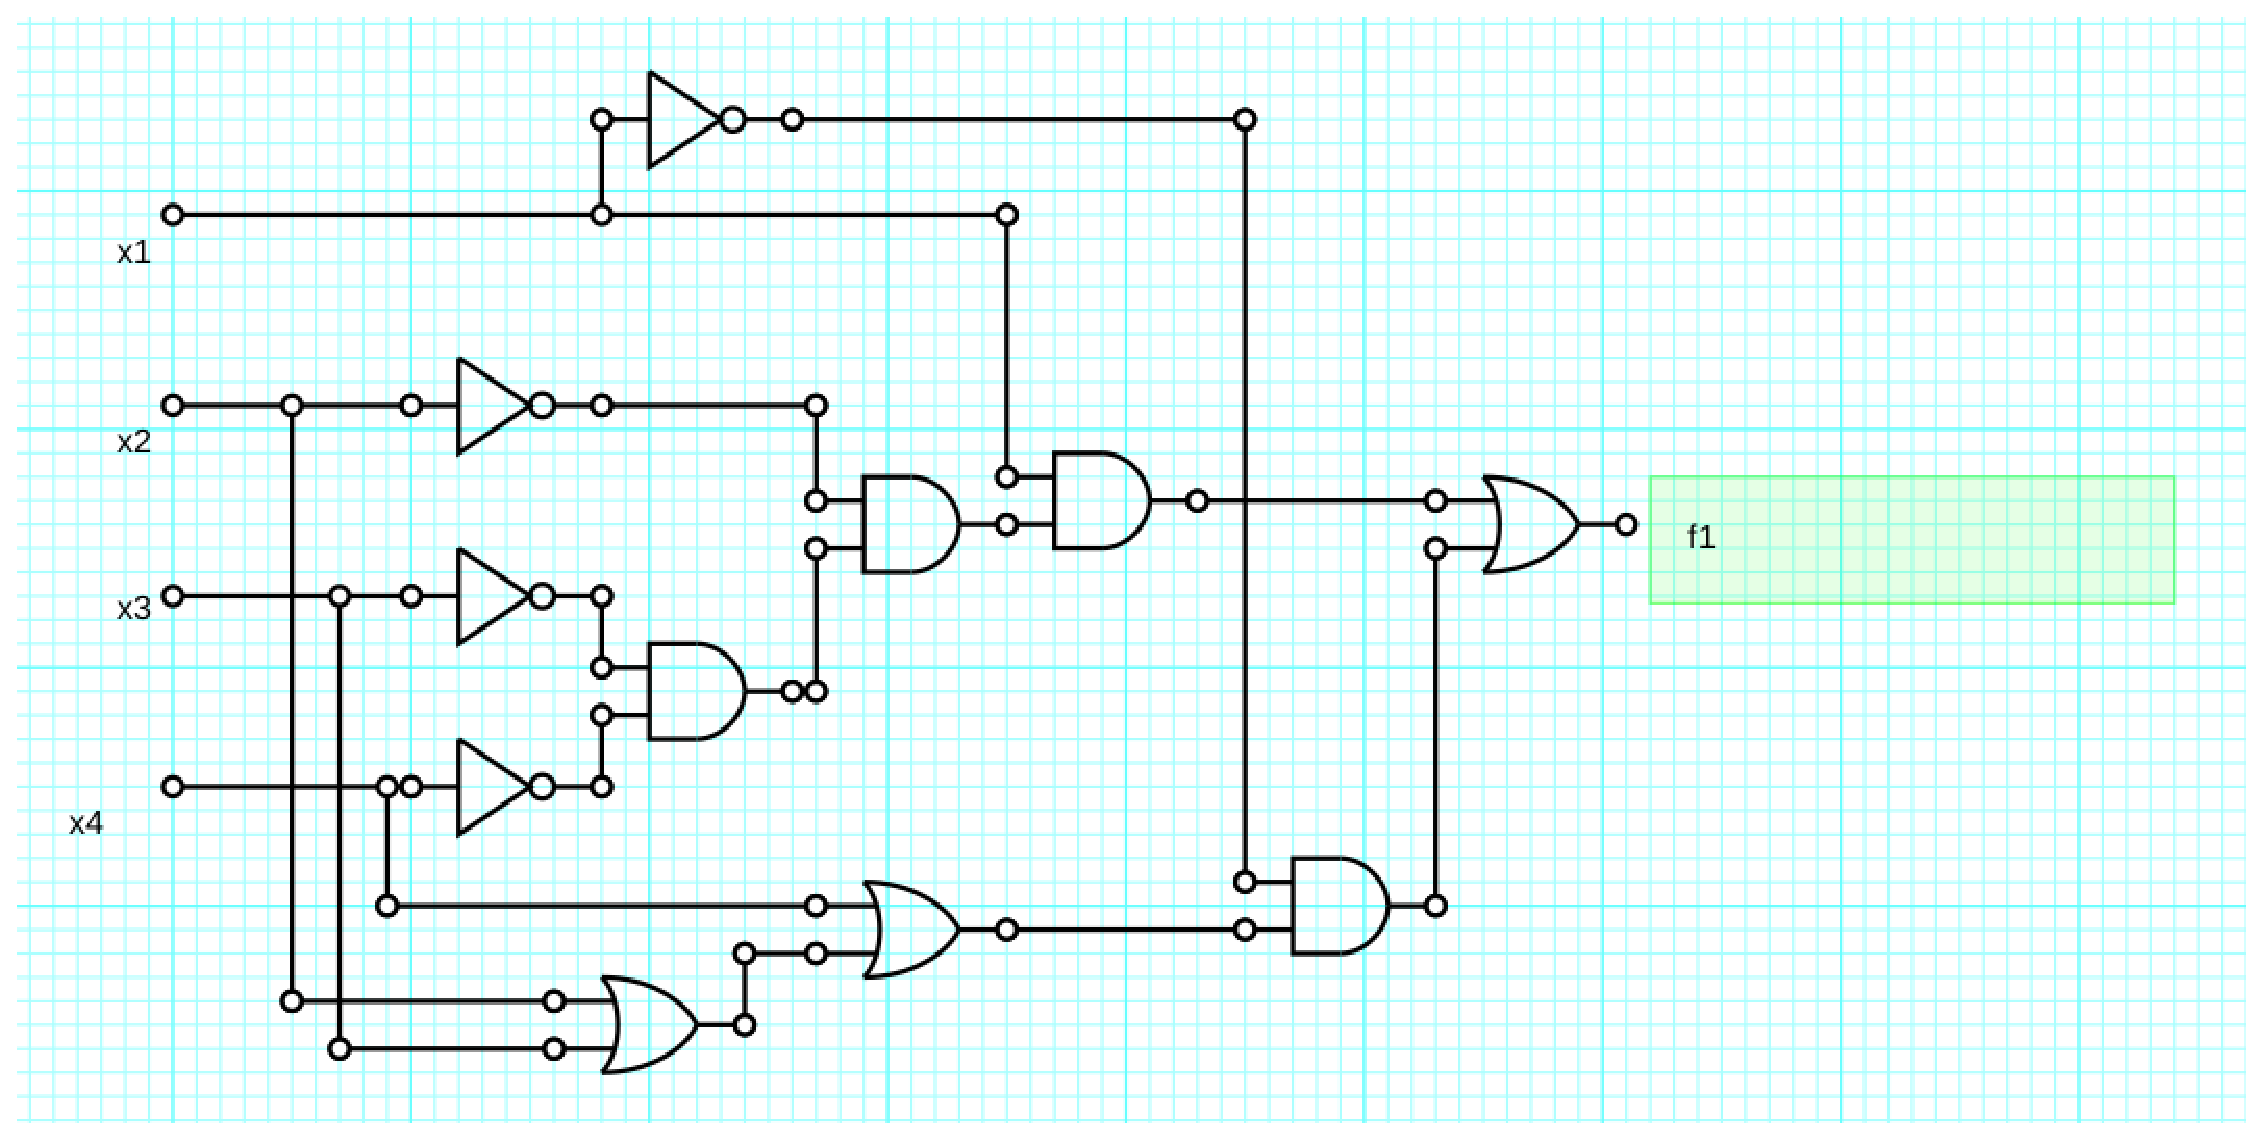
\includegraphics[scale=0.25]{images/1} 
\par\end{centering}
\caption{Grafico de compuertas logicas Bit 1}
\end{figure}

\begin{figure}[H]
\begin{centering}
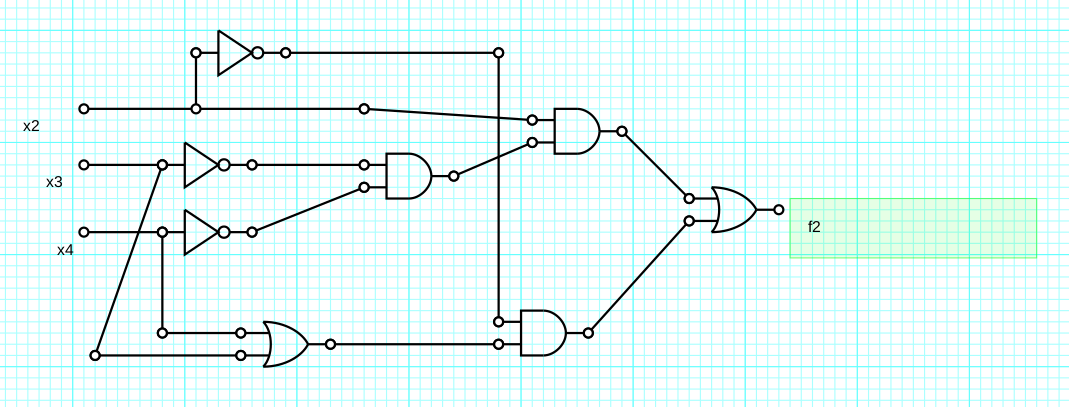
\includegraphics[scale=0.25]{images/2} 
\par\end{centering}
\caption{Grafico de compuertas logicas Bit 2}
\end{figure}

\begin{figure}[H]
\begin{centering}
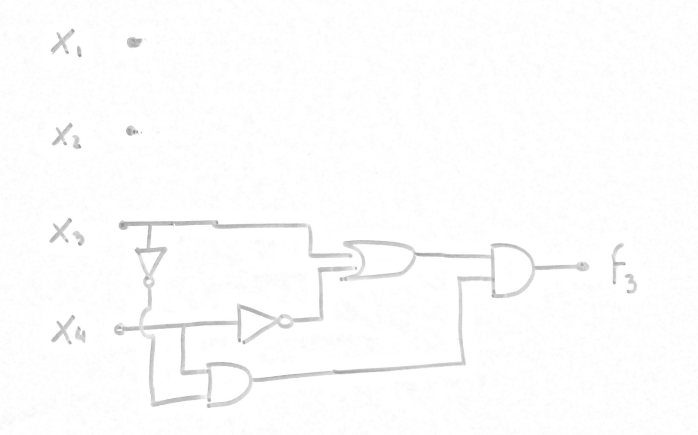
\includegraphics[scale=0.25]{images/3} 
\par\end{centering}
\caption{Grafico de compuertas logicas Bit 3}
\end{figure}

\begin{figure}[H]
\begin{centering}
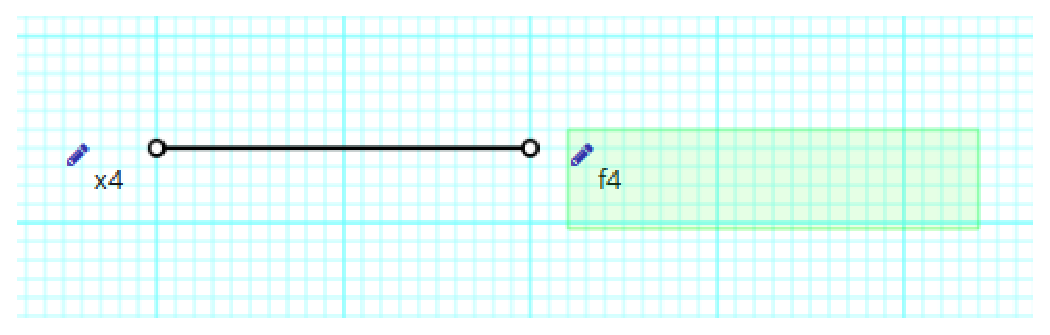
\includegraphics[scale=0.25]{images/4} 
\par\end{centering}
\caption{Grafico de compuertas logicas Bit 4}
\end{figure}

Finalmente, esta logica de compuertas fue implementada en verilog
de la siguiente manera:

\begin{figure}[H]
\begin{centering}
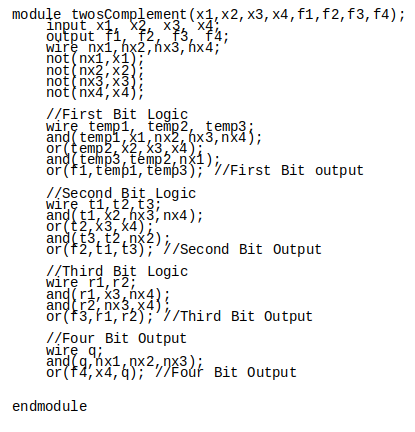
\includegraphics[scale=0.4]{images/5} 
\par\end{centering}
\caption{Implementacion de la logica en Verilog}
\end{figure}

y al probar el codigo con un test.v se obtuvo la siguiente salida,
confirmando que el codigo se realizo de manera exitosa.

\begin{figure}[H]
\begin{centering}
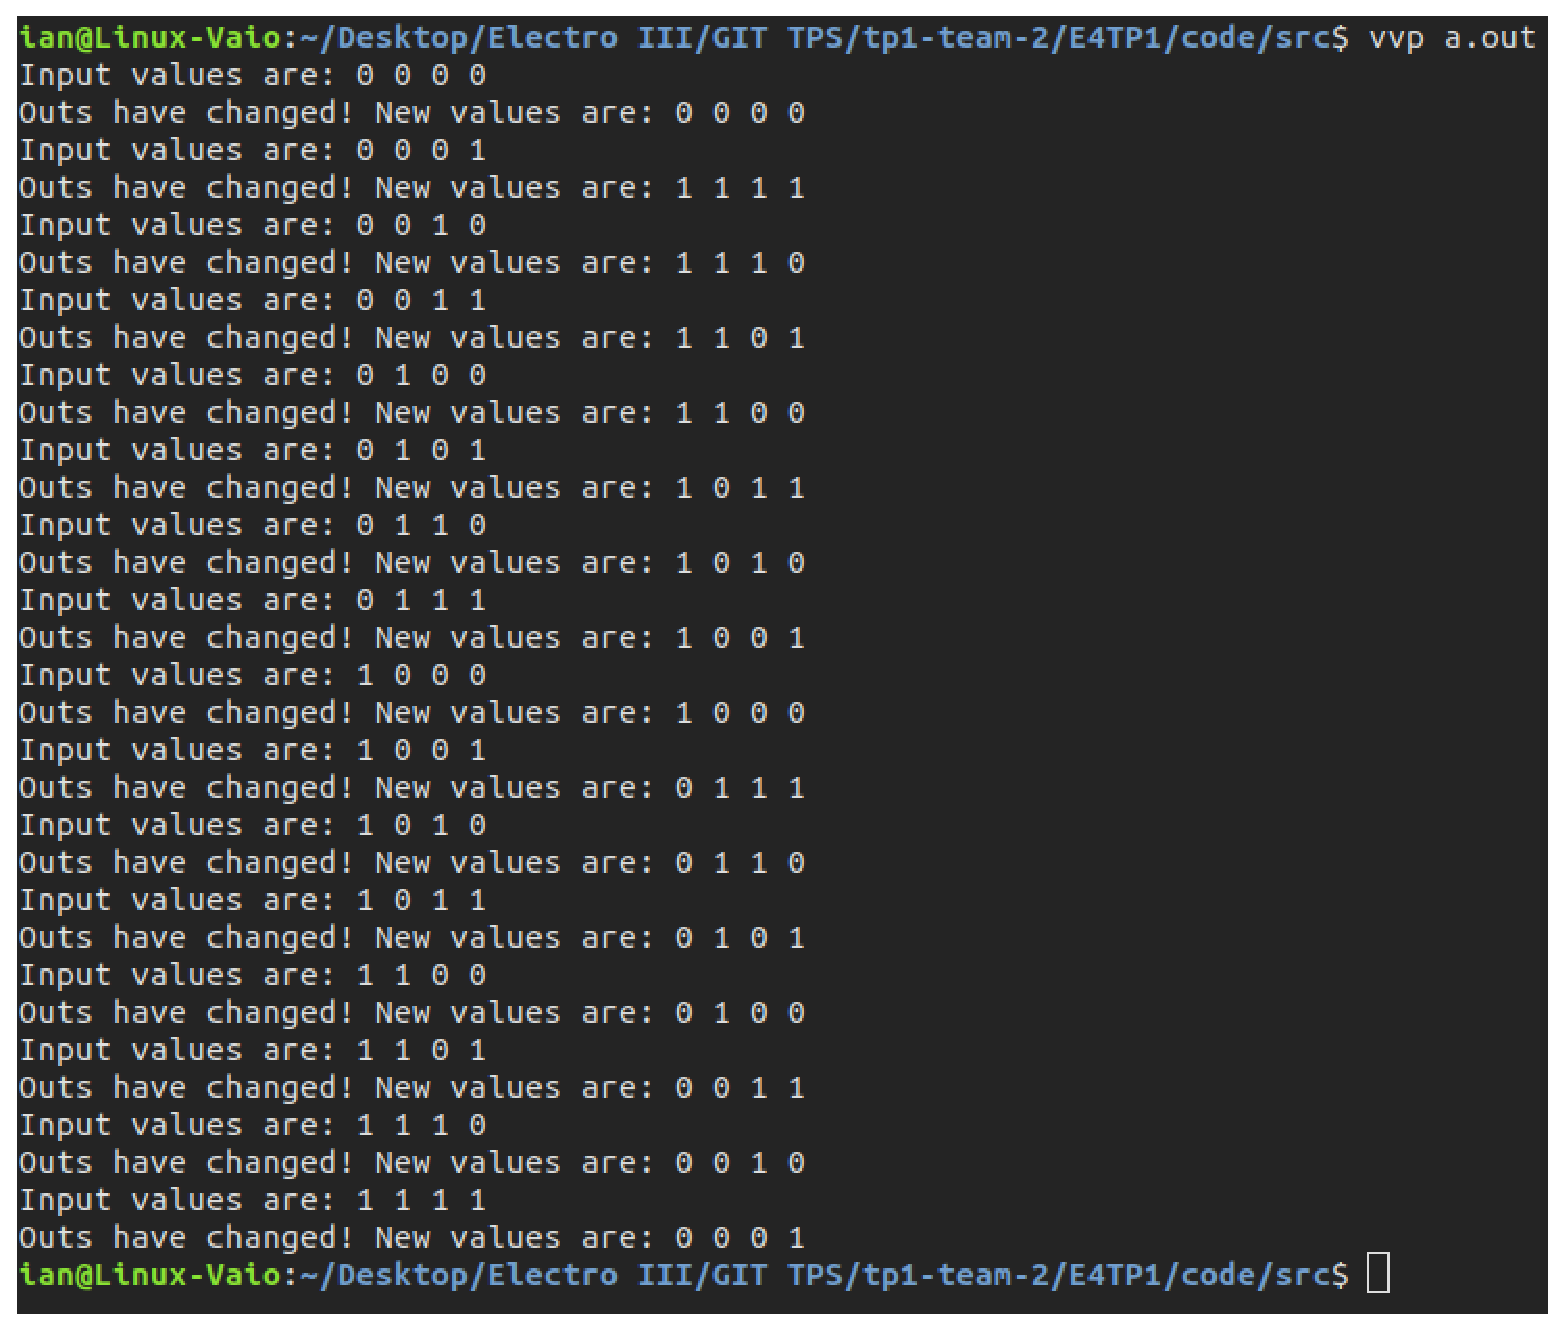
\includegraphics[scale=0.4]{images/6} 
\par\end{centering}
\caption{Salida de la implementacion en la Terminal}
\end{figure}

\end{document}
